\clearpage
\section{Temporal Alternating Direction Method of Multipliers (tADMM)}

\subsection{Introduction and Motivation}

Multi-period optimal power flow (MPOPF) problems are computationally challenging due to the coupling of variables across time periods through energy storage devices, such as batteries. The temporal coupling arises from the state-of-charge (SOC) dynamics, which link the battery's energy level at each time step to its charging/discharging decisions throughout the entire planning horizon. For large-scale distribution networks with multiple time periods, solving the centralized MPOPF problem becomes intractable.

The Alternating Direction Method of Multipliers (ADMM) is a powerful decomposition technique for solving large-scale convex optimization problems~\cite{admm_boyd_website, admm_cmu_notes}. ADMM is particularly effective for problems that can be decomposed into smaller, more manageable subproblems. The temporal ADMM (tADMM) approach adapts the classical ADMM framework to decompose the MPOPF problem across the temporal dimension, enabling parallel computation of individual time-step subproblems while maintaining consensus on the battery SOC trajectories.

The key insight of tADMM is that while spatial network constraints (power flow equations, voltage limits) are local to each time step, the temporal coupling through battery SOC can be handled through consensus variables. Each time-step subproblem maintains its own local copy of the battery SOC trajectory, and these local copies are coordinated through a global consensus variable that is updated iteratively. This decomposition structure allows for:
\begin{itemize}
    \item \textbf{Parallel computation}: Each time-step subproblem can be solved independently and in parallel
    \item \textbf{Scalability}: Computational complexity grows more favorably with the number of time periods compared to centralized approaches
    \item \textbf{Modularity}: The framework can accommodate different network models (LinDistFlow, copper plate) without changing the decomposition structure
\end{itemize}

\subsection{LinDistFlow MPOPF with tADMM}

\subsubsection{Problem Overview}

The Temporal ADMM (tADMM) algorithm decomposes the multi-period optimal power flow problem for distribution networks into $T$ subproblems, each corresponding to one time period. This formulation uses the linearized DistFlow model to capture network physics including voltage drops and reactive power flows. The algorithm maintains consensus on battery state-of-charge (SOC) trajectories across all subproblems through an iterative update procedure.

\subsubsection{Variable Color Coding}

To clearly distinguish the different types of variables in the tADMM formulation, we use the following color-coding scheme:
\begin{itemize}
    \item \textcolor{blue}{$\mathbf{B_j^{t_0}[t]}$ (Blue)}: Local SOC variables for battery $j$ in subproblem $t_0$, evaluated at time $t$. These are the primal variables optimized in each subproblem.
    \item \textcolor{red}{$\mathbf{\hat{B}_j[t]}$ (Red)}: Global consensus SOC for battery $j$ at time $t$. This represents the agreed-upon SOC trajectory that all subproblems aim to converge to.
    \item \textcolor{green!60!black}{$\mathbf{u_j^{t_0}[t]}$ (Green)}: Local scaled dual variables for battery $j$ in subproblem $t_0$, for time $t$. These accumulate the consensus violation and guide convergence.
\end{itemize}

\subsubsection{Sets and Indices}
\begin{itemize}
    \item $\mathcal{N}$: Set of all nodes (buses)
    \item $\mathcal{L}$: Set of all branches (lines)
    \item $\mathcal{L}_1$: Set of branches connected to substation (node 1)
    \item $\mathcal{B}$: Set of nodes with batteries
    \item $\mathcal{D}$: Set of nodes with PV (DER)
    \item $\mathcal{T} = \{1, 2, \ldots, T\}$: Set of time periods
    \item $t_0 \in \mathcal{T}$: Index for a specific time period in tADMM decomposition
    \item $j \in \mathcal{N}$: Node index
    \item $(i,j) \in \mathcal{L}$: Branch from node $i$ to node $j$
\end{itemize}

\subsubsection{tADMM Algorithm Structure}

The tADMM algorithm follows the consensus-based ADMM framework~\cite{admm_boyd_website, admm_cmu_notes}, where the true global problem involves a single consensus variable that is used (partially or fully) by all individual subproblems. In the context of MPOPF, the consensus variable is the battery SOC trajectory, and each time-step subproblem maintains its own local copy of this trajectory.

The algorithm alternates between three update steps at each iteration $k$:

\paragraph{Step 1: Subproblem Update (Blue Variables)}

In the first update step, we solve each subproblem $t_0 \in \{1, 2, \ldots, T\}$ independently and in parallel. Each subproblem optimizes its local copy of the battery SOC trajectory \textcolor{blue}{$\mathbf{B_j^{t_0}[t]}$} along with the network variables for its specific time step. The latest values of the global consensus variable \textcolor{red}{$\mathbf{\hat{B}_j[t]}$} and dual variables \textcolor{green!60!black}{$\mathbf{u_j^{t_0}[t]}$} from the previous iteration are used to guide the optimization toward consensus.

For each subproblem $t_0 \in \{1, 2, \ldots, T\}$:

\begin{align}
\min_{\substack{P_{\text{Subs}}^{t_0}, Q_{\text{Subs}}^{t_0}, \\ P_{ij}^{t_0}, Q_{ij}^{t_0}, v_j^{t_0}, q_{D,j}^{t_0}, \\ P_{B,j}^t, \textcolor{blue}{\mathbf{B_j^{t_0}[t]}} \\ \forall j \in \mathcal{B}, \, t \in \mathcal{T}}} \quad & c^{t_0} \cdot P_{\text{Subs}}^{t_0} \cdot P_{\text{BASE}} \cdot \Delta t + C_B \sum_{j \in \mathcal{B}} \left(P_{B,j}^{t_0}\right)^2 \cdot P_{\text{BASE}}^2 \cdot \Delta t \notag \\
& + \frac{\rho}{2} \sum_{j \in \mathcal{B}} \sum_{t=1}^T \left( \textcolor{blue}{\mathbf{B_j^{t_0}[t]}} - \textcolor{red}{\mathbf{\hat{B}_j[t]}} + \textcolor{green!60!black}{\mathbf{u_j^{t_0}[t]}} \right)^2
\end{align}

\textbf{Subject to:}

\textbf{Spatial Network Constraints (only for time $t_0$):}
\begin{align}
\text{Real power balance (substation):} \quad & P_{\text{Subs}}^{t_0} - \sum_{(1,j) \in \mathcal{L}_1} P_{1j}^{t_0} = 0 \\
\text{Real power balance (nodes):} \quad & P_{ij}^{t_0} - \sum_{(j,k) \in \mathcal{L}} P_{jk}^{t_0} = P_{B,j}^{t_0} + p_{D,j}^{t_0} - p_{L,j}^{t_0}, \notag \\
& \quad \forall (i,j) \in \mathcal{L}, \\
\text{Reactive power balance (substation):} \quad & Q_{\text{Subs}}^{t_0} - \sum_{(1,j) \in \mathcal{L}_1} Q_{1j}^{t_0} = 0 \\
\text{Reactive power balance (nodes):} \quad & Q_{ij}^{t_0} - \sum_{(j,k) \in \mathcal{L}} Q_{jk}^{t_0} = q_{D,j}^{t_0} - q_{L,j}^{t_0}, \notag \\
& \quad \forall (i,j) \in \mathcal{L}, \\
\text{KVL constraints:} \quad & v_i^{t_0} - v_j^{t_0} = 2(r_{ij} P_{ij}^{t_0} + x_{ij} Q_{ij}^{t_0}), \quad \forall (i,j) \in \mathcal{L} \\
\text{Voltage limits:} \quad & (V_{\min,j})^2 \leq v_j^{t_0} \leq (V_{\max,j})^2, \quad \forall j \in \mathcal{N} \\
\text{PV reactive limits:} \quad & -\sqrt{(S_{D,j})^2 - (p_{D,j}^{t_0})^2} \leq q_{D,j}^{t_0} \leq \sqrt{(S_{D,j})^2 - (p_{D,j}^{t_0})^2}, \notag \\
& \quad \forall j \in \mathcal{D}
\end{align}

\textbf{Temporal Battery Constraints (entire horizon $t \in \{1, \ldots, T\}$):}
\begin{align}
\text{Initial SOC:} \quad & \textcolor{blue}{\mathbf{B_j^{t_0}[1]}} = B_{0,j} - P_{B,j}^1 \cdot \Delta t, \quad \forall j \in \mathcal{B} \\
\text{SOC trajectory:} \quad & \textcolor{blue}{\mathbf{B_j^{t_0}[t]}} = \textcolor{blue}{\mathbf{B_j^{t_0}[t-1]}} - P_{B,j}^t \cdot \Delta t, \quad \forall t \in \{2, \ldots, T\}, \, j \in \mathcal{B} \\
\text{SOC limits:} \quad & \text{SOC}_{\min,j} \cdot B_{\text{rated},j} \leq \textcolor{blue}{\mathbf{B_j^{t_0}[t]}} \leq \text{SOC}_{\max,j} \cdot B_{\text{rated},j}, \notag \\
& \quad \forall t \in \mathcal{T}, \, j \in \mathcal{B} \\
\text{Power limits:} \quad & -P_{B,\text{rated},j} \leq P_{B,j}^t \leq P_{B,\text{rated},j}, \quad \forall t \in \mathcal{T}, \, j \in \mathcal{B}
\end{align}

\textbf{Key Formulation Notes:}
\begin{itemize}
    \item \textbf{Network variables} $(P_{\text{Subs}}^{t_0}, Q_{\text{Subs}}^{t_0}, P_{ij}^{t_0}, Q_{ij}^{t_0}, v_j^{t_0}, q_{D,j}^{t_0})$ are optimized \textit{only} for time step $t_0$, representing the spatial network state at that particular time
    \item \textbf{Battery power} $P_{B,j}^t$ is optimized for the \textit{entire} horizon $t \in \{1, \ldots, T\}$ to allow proper accounting of temporal coupling
    \item \textbf{Local SOC trajectory} \textcolor{blue}{$\mathbf{B_j^{t_0}[t]}$} is computed for \textit{all} time steps $t \in \{1, \ldots, T\}$ based on the battery power decisions
    \item The ADMM consensus penalty compares the full local trajectory \textcolor{blue}{$\mathbf{B_j^{t_0}[t]}$} with the global master copy \textcolor{red}{$\mathbf{\hat{B}_j[t]}$}, penalized by the dual variables \textcolor{green!60!black}{$\mathbf{u_j^{t_0}[t]}$}
    \item Each battery $j \in \mathcal{B}$ has its own set of local/global SOC variables and dual variables
\end{itemize}

\paragraph{Step 2: Consensus Update (Red Variables)}

After all subproblems have been solved in parallel to obtain the latest values of \textcolor{blue}{$\mathbf{B_j^{t_0}[t]}$}, the global consensus variable \textcolor{red}{$\mathbf{\hat{B}_j[t]}$} is updated by averaging the local SOC trajectories across all subproblems, adjusted by the dual variables. This update brings the consensus closer to the average of what each subproblem believes the SOC should be.

For each battery $j \in \mathcal{B}$ and each time period $t \in \mathcal{T}$:
\begin{align}
\textcolor{red}{\mathbf{\hat{B}_j[t]}} &= \text{clamp}\left( \frac{1}{T} \sum_{t_0=1}^{T} \left( \textcolor{blue}{\mathbf{B_j^{t_0}[t]}} + \textcolor{green!60!black}{\mathbf{u_j^{t_0}[t]}} \right), \underline{B}_j, \overline{B}_j \right)
\end{align}

where $\underline{B}_j = \text{SOC}_{\min,j} \cdot B_{\text{rated},j}$ and $\overline{B}_j = \text{SOC}_{\max,j} \cdot B_{\text{rated},j}$. The clamping operation ensures that the consensus variable respects the physical SOC bounds.

\paragraph{Step 3: Dual Update (Green Variables)}

Finally, the dual variables \textcolor{green!60!black}{$\mathbf{u_j^{t_0}[t]}$} are updated to accumulate the consensus violation (the difference between local and global SOC). These dual variables act as Lagrange multipliers that enforce consensus in the limit as the algorithm converges.

For each battery $j \in \mathcal{B}$, each subproblem $t_0 \in \mathcal{T}$, and each time period $t \in \mathcal{T}$:
\begin{align}
\textcolor{green!60!black}{\mathbf{u_j^{t_0}[t]}} &:= \textcolor{green!60!black}{\mathbf{u_j^{t_0}[t]}} + \left( \textcolor{blue}{\mathbf{B_j^{t_0}[t]}} - \textcolor{red}{\mathbf{\hat{B}_j[t]}} \right)
\end{align}

These three steps are repeated iteratively: solve subproblems for \textcolor{blue}{blue variables}, update consensus \textcolor{red}{red variables}, and update dual \textcolor{green!60!black}{green variables}, until convergence is achieved.

\subsubsection{Convergence Criteria}

\textbf{Primal Residual (Consensus Violation):}

The primal residual measures how well the local SOC trajectories \textcolor{blue}{$\mathbf{B_j^{t_0}[t]}$} agree with the global consensus \textcolor{red}{$\mathbf{\hat{B}_j[t]}$} across all batteries and time steps.

\begin{align}
\|r^k\|_2 &= \frac{1}{|\mathcal{B}|} \sqrt{\sum_{j \in \mathcal{B}} \sum_{t=1}^T \left( \frac{1}{T} \sum_{t_0=1}^T \textcolor{blue}{\mathbf{B_j^{t_0}[t]}} - \textcolor{red}{\mathbf{\hat{B}_j[t]}} \right)^2} \leq \epsilon_{\text{pri}}
\end{align}

\textbf{Dual Residual (Consensus Change):}

The dual residual measures the change in the consensus variable between iterations, indicating convergence stability.

\begin{align}
\|s^k\|_2 &= \frac{\rho}{|\mathcal{B}|} \sqrt{\sum_{j \in \mathcal{B}} \sum_{t=1}^T \left( \textcolor{red}{\mathbf{\hat{B}_j^k[t]}} - \textcolor{red}{\mathbf{\hat{B}_j^{k-1}[t]}} \right)^2} \leq \epsilon_{\text{dual}}
\end{align}

\subsection{Copper Plate MPOPF with tADMM (Simplified Case)}

\subsubsection{Problem Overview}

To illustrate the tADMM framework more clearly, we first present a simplified copper plate model where network constraints are neglected, and only a single aggregate power balance is enforced at each time step. The Temporal ADMM (tADMM) algorithm decomposes the multi-period optimal power flow problem into $T$ single-step subproblems, each corresponding to one time period. The hope is to enable parallel computation and improved scalability while still retaining solution optimality. Fig.~\ref{fig:input_curves} shows the input data for a 24-hour horizon, including the time-varying electricity cost and load demand profiles used in the copper plate MPOPF formulation.

\begin{figure}[h]
    \centering
    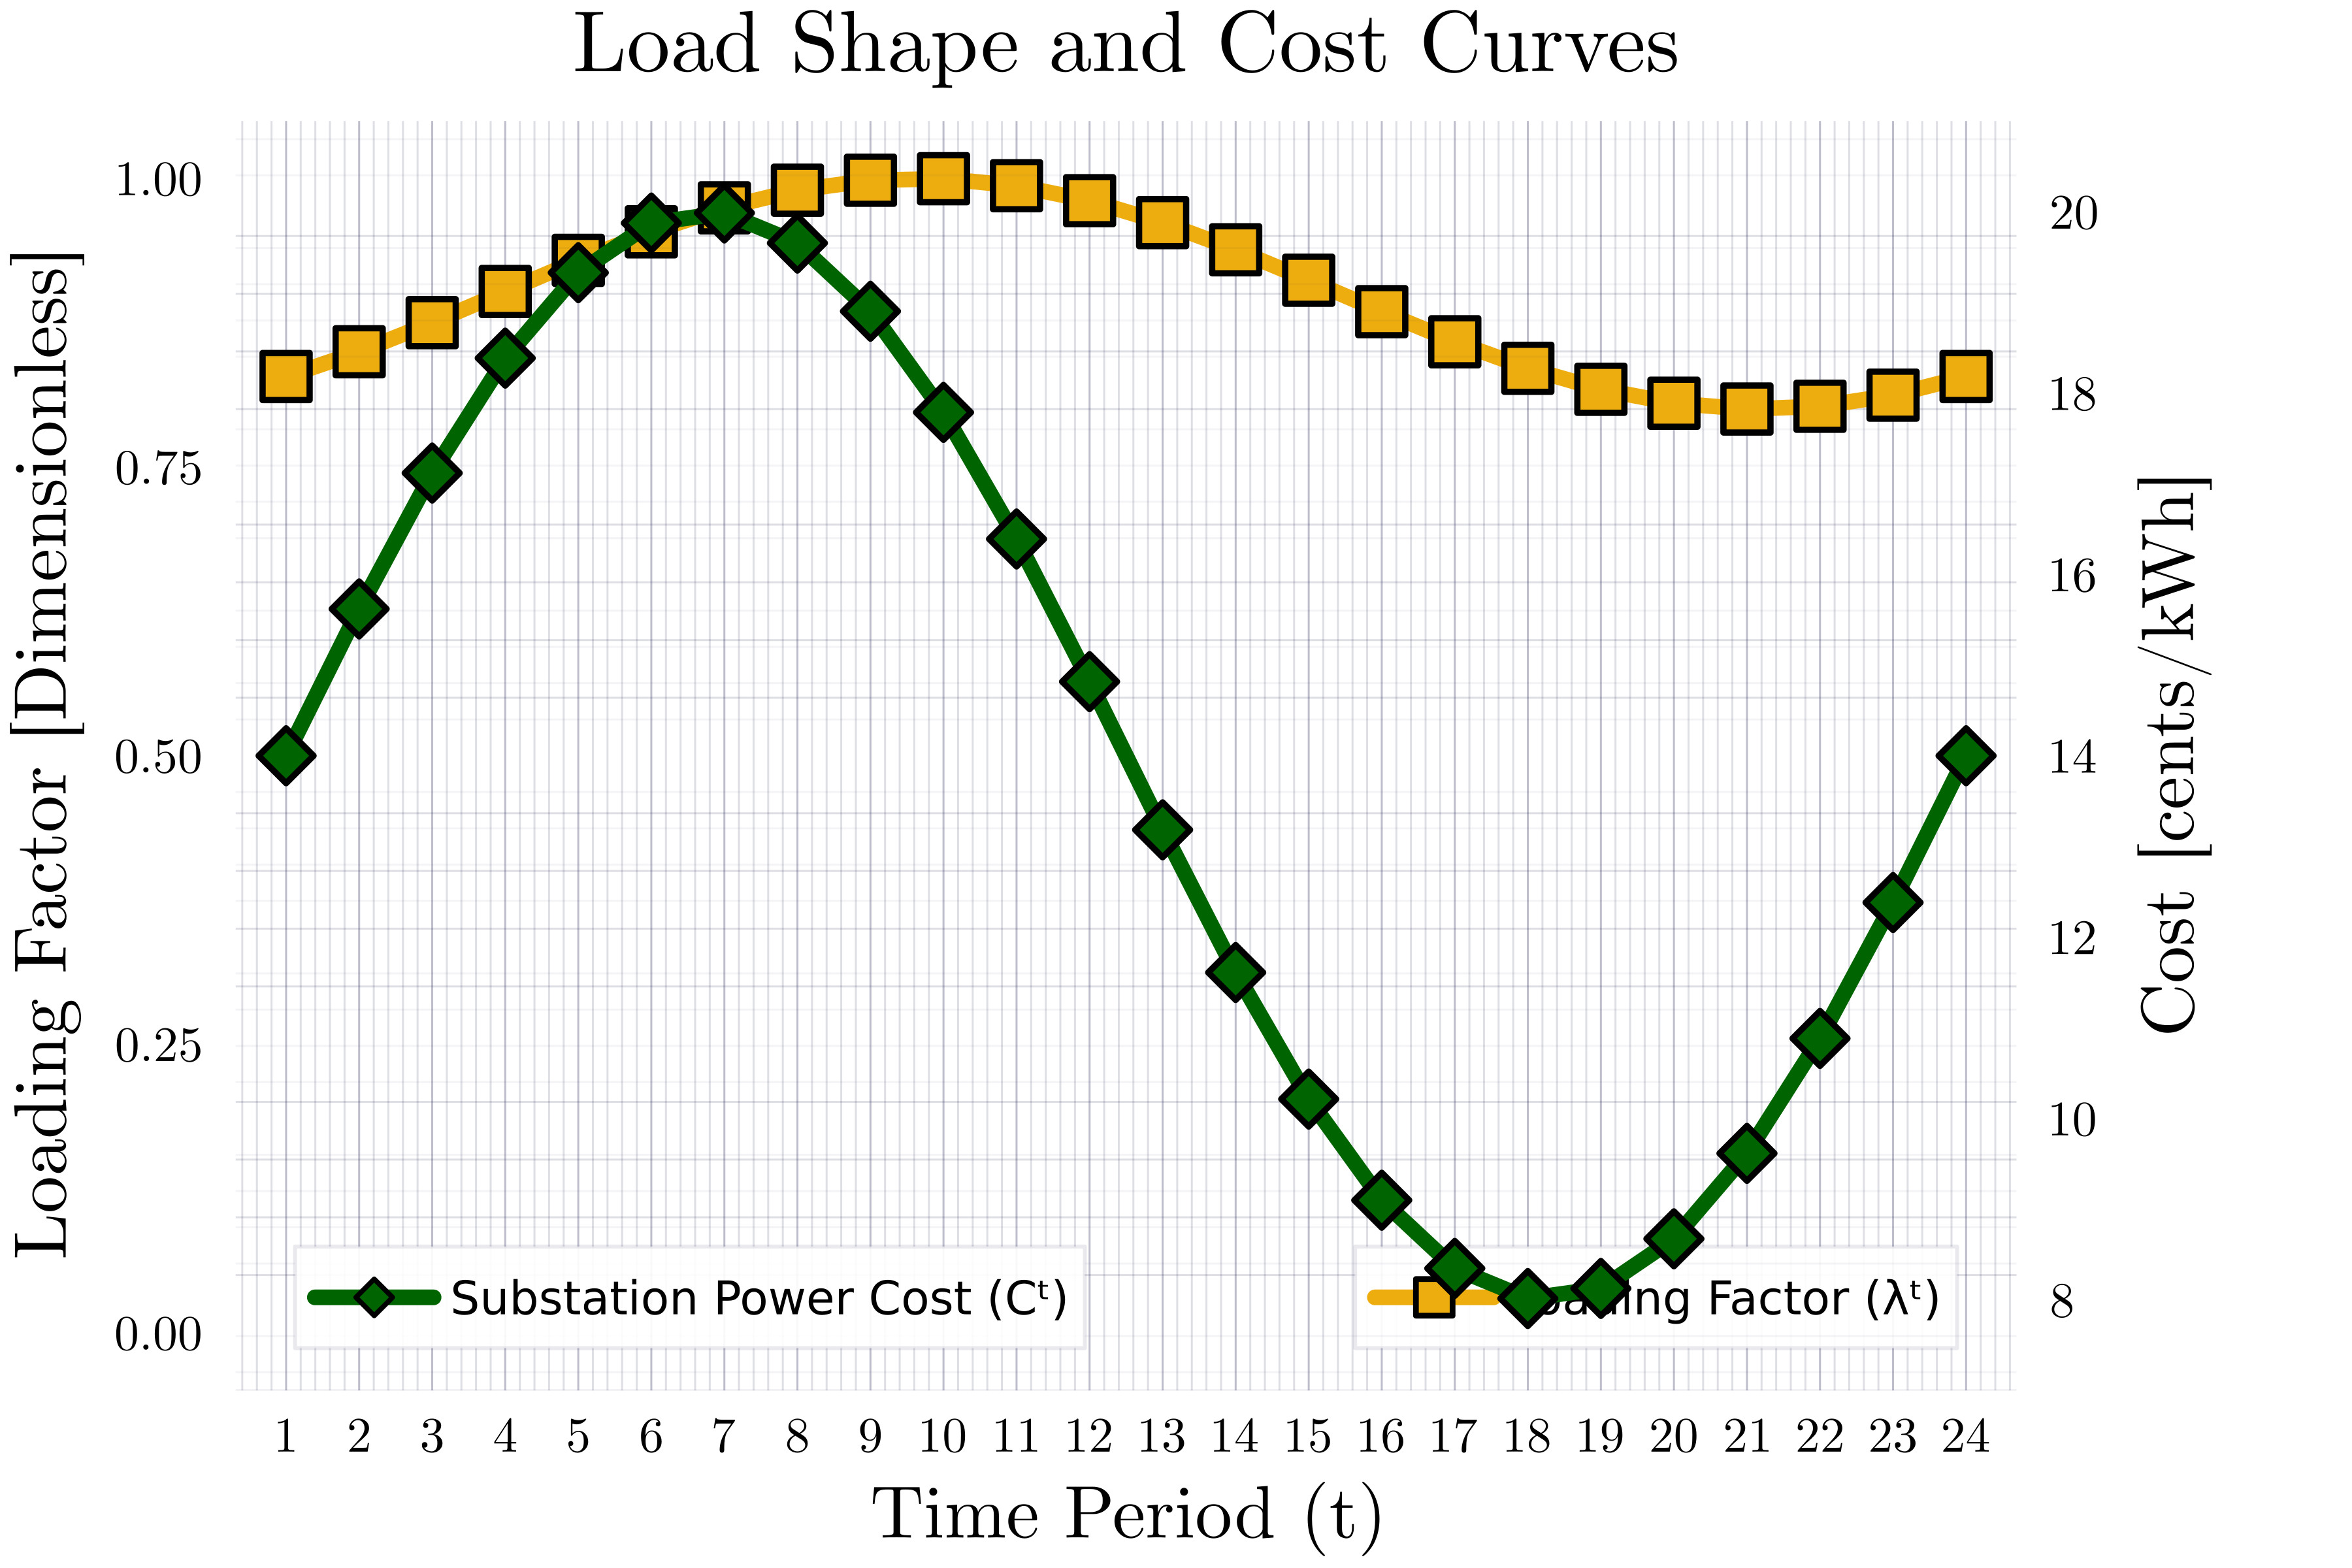
\includegraphics[width=0.7\textwidth]{figures/input-curves-cost-and-load-only-T24.png}
    \caption{Input curves showing electricity cost and load demand over a 24-hour period.}
    \label{fig:input_curves}
\end{figure}

\subsubsection{Variable Color Coding}
\begin{itemize}
    \item \textcolor{blue}{$\mathbf{B^{t_0}}$ (Blue)}: Local SOC variables for subproblem $t_0$
    \item \textcolor{red}{$\mathbf{\hat{B}}$ (Red)}: Global consensus SOC trajectory
    \item \textcolor{green!60!black}{$\mathbf{u^{t_0}}$ (Green)}: Local scaled dual variables for subproblem $t_0$
\end{itemize}

\subsubsection{tADMM Algorithm Structure}

The algorithm alternates between three update steps following the consensus ADMM framework~\cite{admm_boyd_website, admm_cmu_notes}:

\paragraph{Step 1: Primal Update (Blue Variables) - tADMM Optimization Model}

In Update 1 (at iteration $k$), the latest values of subproblem copies are solved for in parallel using the last known copies of the consensus variable and dual variables -- namely \textcolor{red}{$\mathbf{\hat{B}^{k-1}}$} and \textcolor{green!60!black}{$\mathbf{u^{t_0, k-1}}$}, respectively.

For each subproblem $t_0 \in \{1, 2, \ldots, T\}$:

\begin{align}
\min_{P_{\text{subs}}^{t_0}, P_{B}^{t_0}, \textcolor{blue}{\mathbf{B^{t_0}}}} \quad & C^{t_0} \cdot P_{\text{subs}}^{t_0} + C_B \cdot \left(P_{B}^{t_0}\right)^2 + \frac{\rho}{2} \left\| \textcolor{blue}{\mathbf{B^{t_0}}} - \textcolor{red}{\mathbf{\hat{B}}} + \textcolor{green!60!black}{\mathbf{u^{t_0}}} \right\|_2^2
\end{align}

\textbf{Subject to SOC Dynamics for Entire Trajectory:}
\begin{align}
\textcolor{blue}{\mathbf{B^{t_0}[1]}} &= B_0 - P_{B}^{t_0} \cdot \Delta t \\
\textcolor{blue}{\mathbf{B^{t_0}[t]}} &= \textcolor{blue}{\mathbf{B^{t_0}[t-1]}} - P_{B}^{t_0} \cdot \Delta t, \quad \forall t \in \{2, \ldots, T\} \\
P_{\text{subs}}^{t_0} + P_{B}^{t_0} &= P_L[t_0] \\
-P_{B,R} \leq P_{B}^{t_0} &\leq P_{B,R} \\
\underline{B} \leq \textcolor{blue}{\mathbf{B^{t_0}[t]}} &\leq \overline{B}, \quad \forall t \in \{1, \ldots, T\}
\end{align}

\textbf{Key Formulation Notes:}
\begin{itemize}
    \item Each subproblem $t_0$ optimizes the battery power $P_{B}^{t_0}$ for \textit{only} time step $t_0$
    \item However, the SOC trajectory \textcolor{blue}{$\mathbf{B^{t_0}[t]}$} is computed for \textit{all} time steps $t \in \{1, \ldots, T\}$
    \item This ensures that the ADMM penalty term can compare the full trajectory \textcolor{blue}{$\mathbf{B^{t_0}}$} with the consensus \textcolor{red}{$\mathbf{\hat{B}}$}
    \item The power balance constraint is enforced only for the specific time $t_0$
\end{itemize}

\paragraph{Step 2: Consensus Update (Red Variables)}

In Update 2 (at iteration $k$), the latest value of the global consensus variable is computed using the last known copies of the local subproblem SOC trajectories and dual variables -- namely \textcolor{blue}{$\mathbf{B_i^{t_0, k}}$} and \textcolor{green!60!black}{$\mathbf{u_i^{t_0, k-1}}$}, respectively.

\begin{align}
\textcolor{red}{\mathbf{\hat{B}[t]}} &= \text{clamp}\left( \frac{1}{T} \sum_{t_0=1}^{T} \left( \textcolor{blue}{\mathbf{B^{t_0}[t]}} + \textcolor{green!60!black}{\mathbf{u^{t_0}[t]}} \right), \underline{B}, \overline{B} \right) \\
&\quad \forall t \in \{1, 2, \ldots, T-1\} \\
\textcolor{red}{\mathbf{\hat{B}[T]}} &= B_{T,\text{target}} \quad \text{(if terminal constraint exists)}
\end{align}

\paragraph{Step 3: Dual Update (Green Variables)}

In Update 3 (at iteration $k$), the latest values of local dual variables are computed using the last known copies of the local SOC, global consensus, and previous dual variables -- namely \textcolor{blue}{$\mathbf{B_i^{t_0, k}}$}, \textcolor{red}{$\mathbf{\hat{B}^k}$}, and \textcolor{green!60!black}{$\mathbf{u_i^{t_0, k-1}}$}, respectively.

\begin{align}
\textcolor{green!60!black}{\mathbf{u^{t_0}[t]}} &:= \textcolor{green!60!black}{\mathbf{u^{t_0}[t]}} + \left( \textcolor{blue}{\mathbf{B^{t_0}[t]}} - \textcolor{red}{\mathbf{\hat{B}[t]}} \right) \\
&\quad \forall t_0 \in \{1, \ldots, T\}, \, \forall t \in \{1, \ldots, T\}
\end{align}

After every subproblem is solved once to get the latest values of \textcolor{blue}{$\mathbf{B_1, B_2, \ldots, B_B}$}, the value of the consensus variable \textcolor{red}{$\mathbf{\hat{B}}$} is updated. Next, the dual variables \textcolor{green!60!black}{$\mathbf{u_1, u_2, \ldots, u_B}$} are updated. This process repeats until convergence.

\subsection{Numerical Results}

\subsubsection{Battery Actions and Convergence Analysis}

To validate the tADMM approach, we present numerical results for the copper plate MPOPF problem with a 24-hour planning horizon. The test case includes a single battery energy storage system with time-varying electricity prices and load demands as shown in Fig.~\ref{fig:input_curves}.

Fig.~\ref{fig:battery_actions_copper_plate} shows the optimal battery charging and discharging actions obtained from solving the centralized (brute force) MPOPF problem. The battery strategically charges during low-cost periods (typically during nighttime and early morning hours) and discharges during high-cost periods (peak demand hours in the afternoon and evening) to minimize the overall energy cost over the 24-hour horizon. This behavior demonstrates the value of energy arbitrage enabled by battery storage.

\begin{figure}[h]
    \centering
    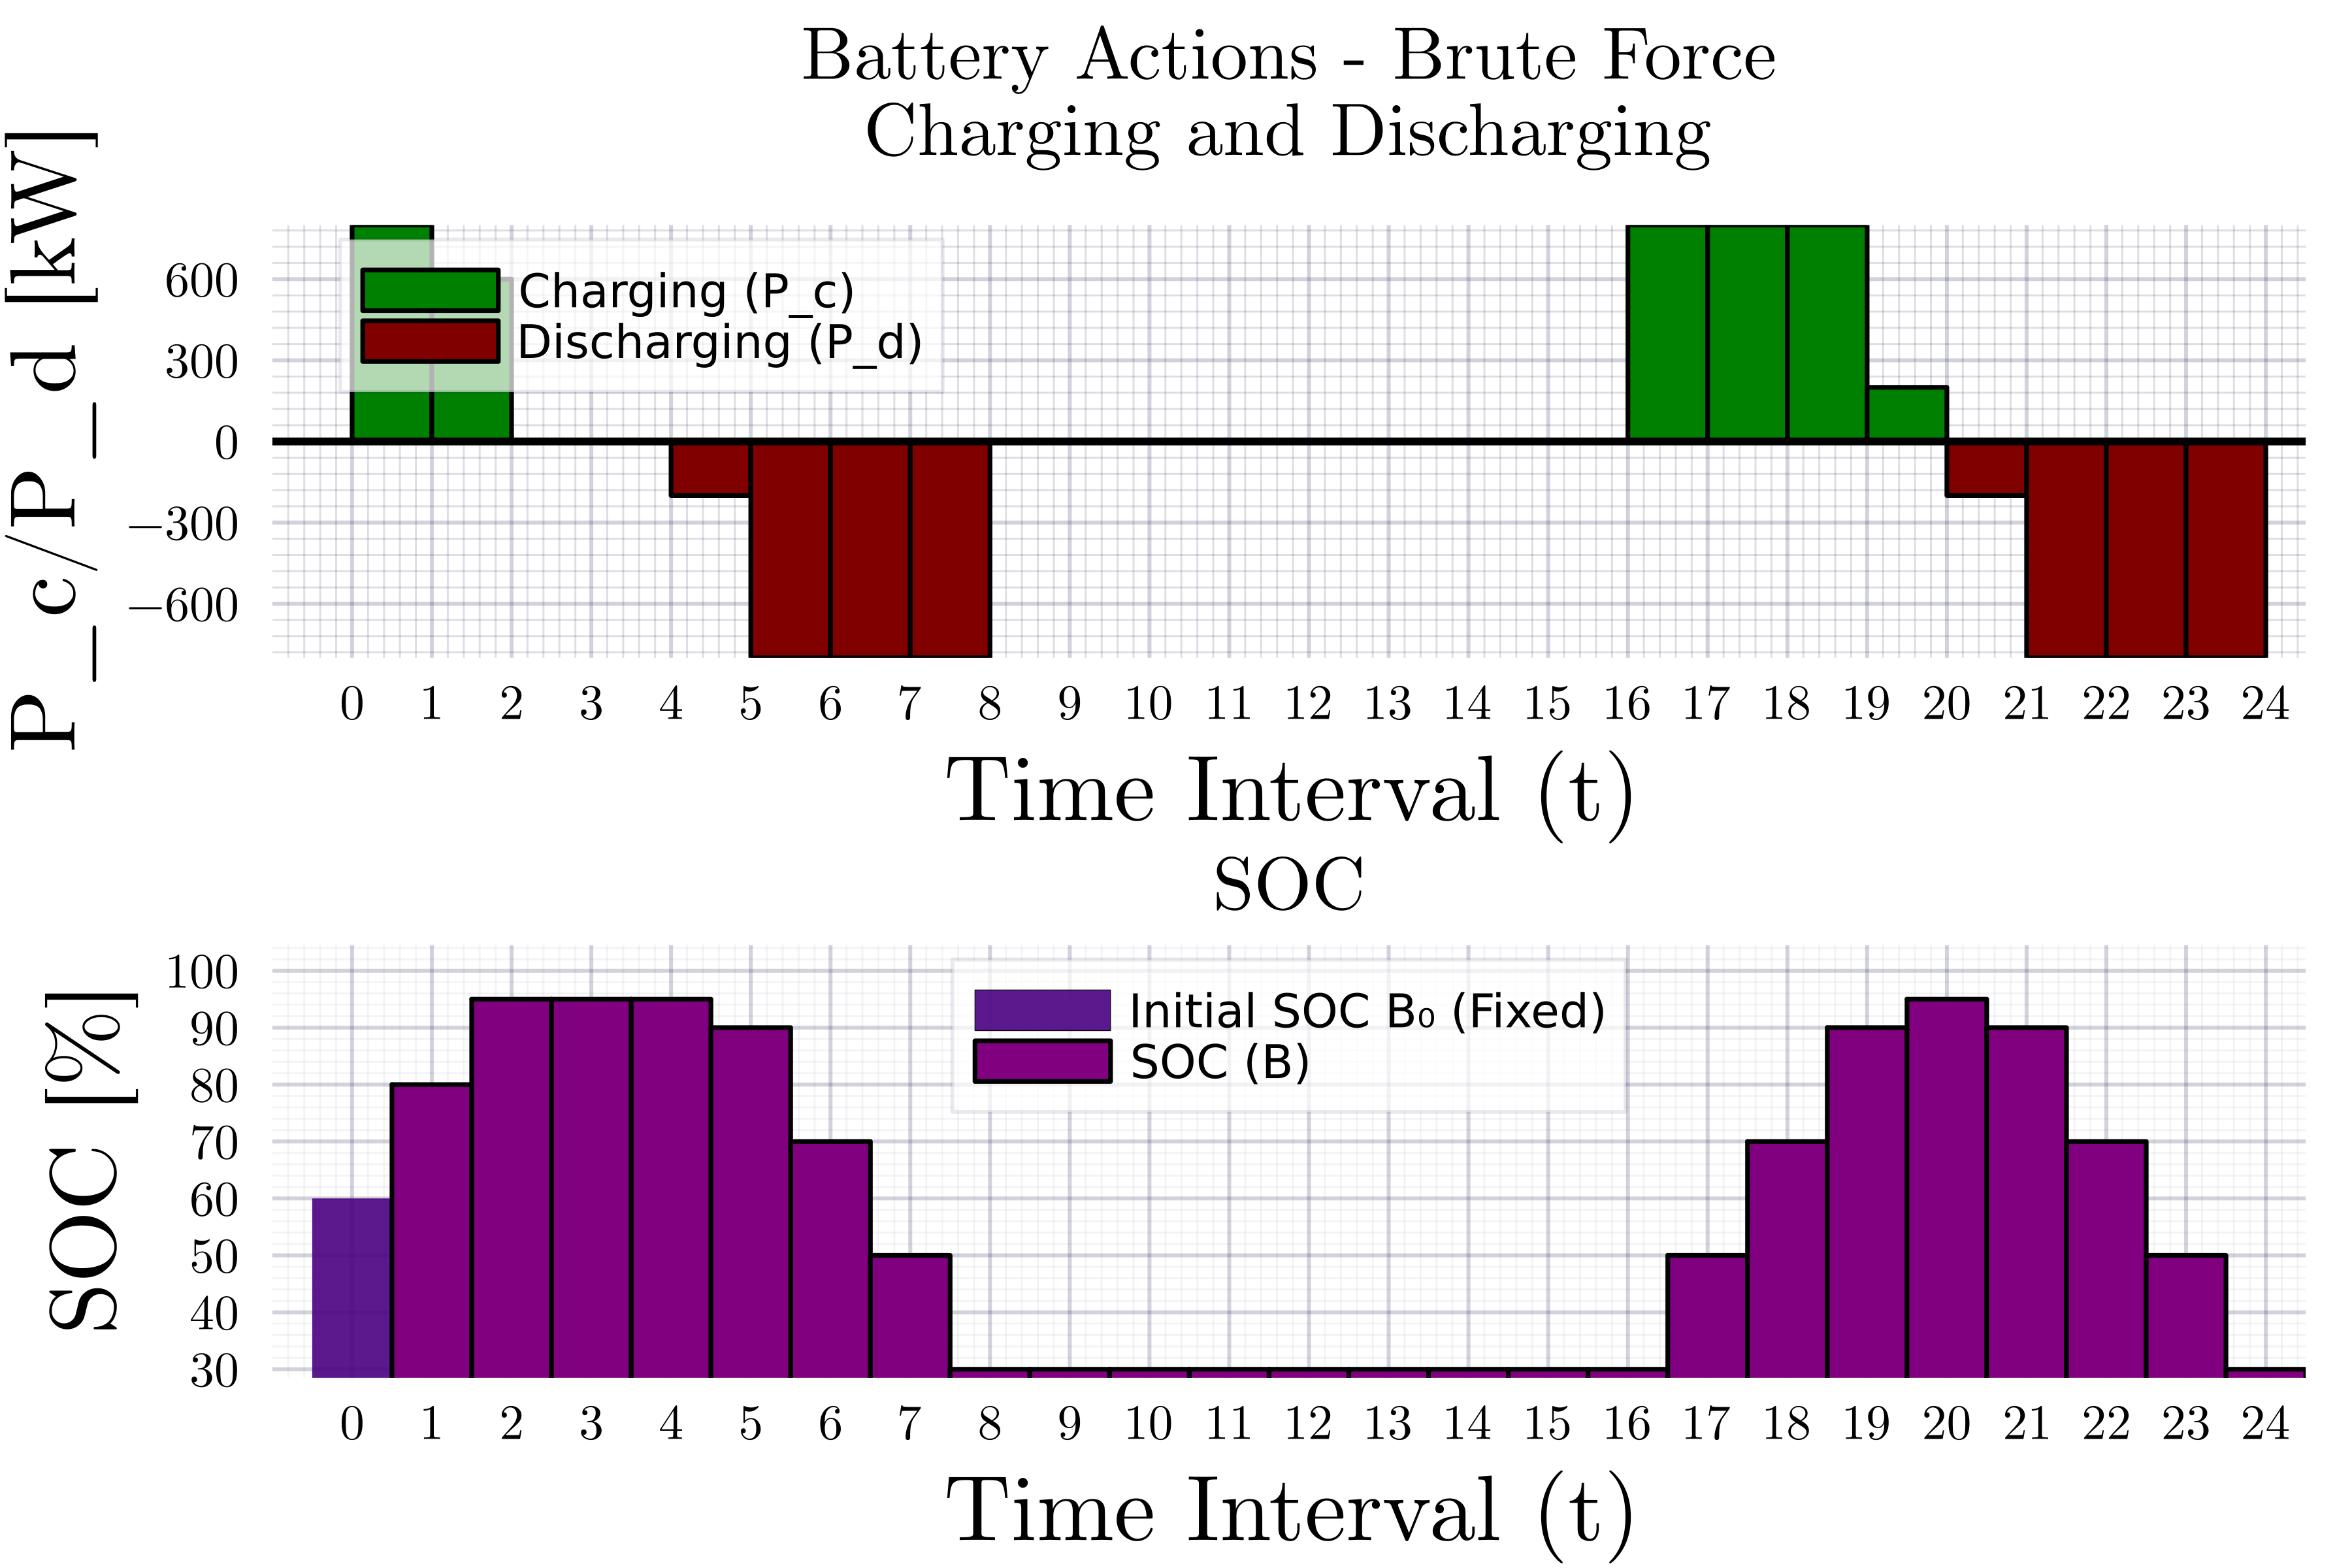
\includegraphics[width=0.7\textwidth]{figures/battery-actions-copper-plate-T24-bf.png}
    \caption{Optimal battery power actions (brute force centralized solution) for copper plate MPOPF over 24-hour horizon. Positive values indicate discharging (supplying power), while negative values indicate charging (consuming power).}
    \label{fig:battery_actions_copper_plate}
\end{figure}

Fig.~\ref{fig:battery_actions_tadmm} presents the battery actions obtained using the tADMM algorithm, demonstrating that the decomposition approach converges to a solution that closely matches the centralized optimal solution. The close agreement between the two solutions validates the effectiveness of the tADMM decomposition for this problem class. Minor differences, if any, are within the specified convergence tolerances.

\begin{figure}[h]
    \centering
    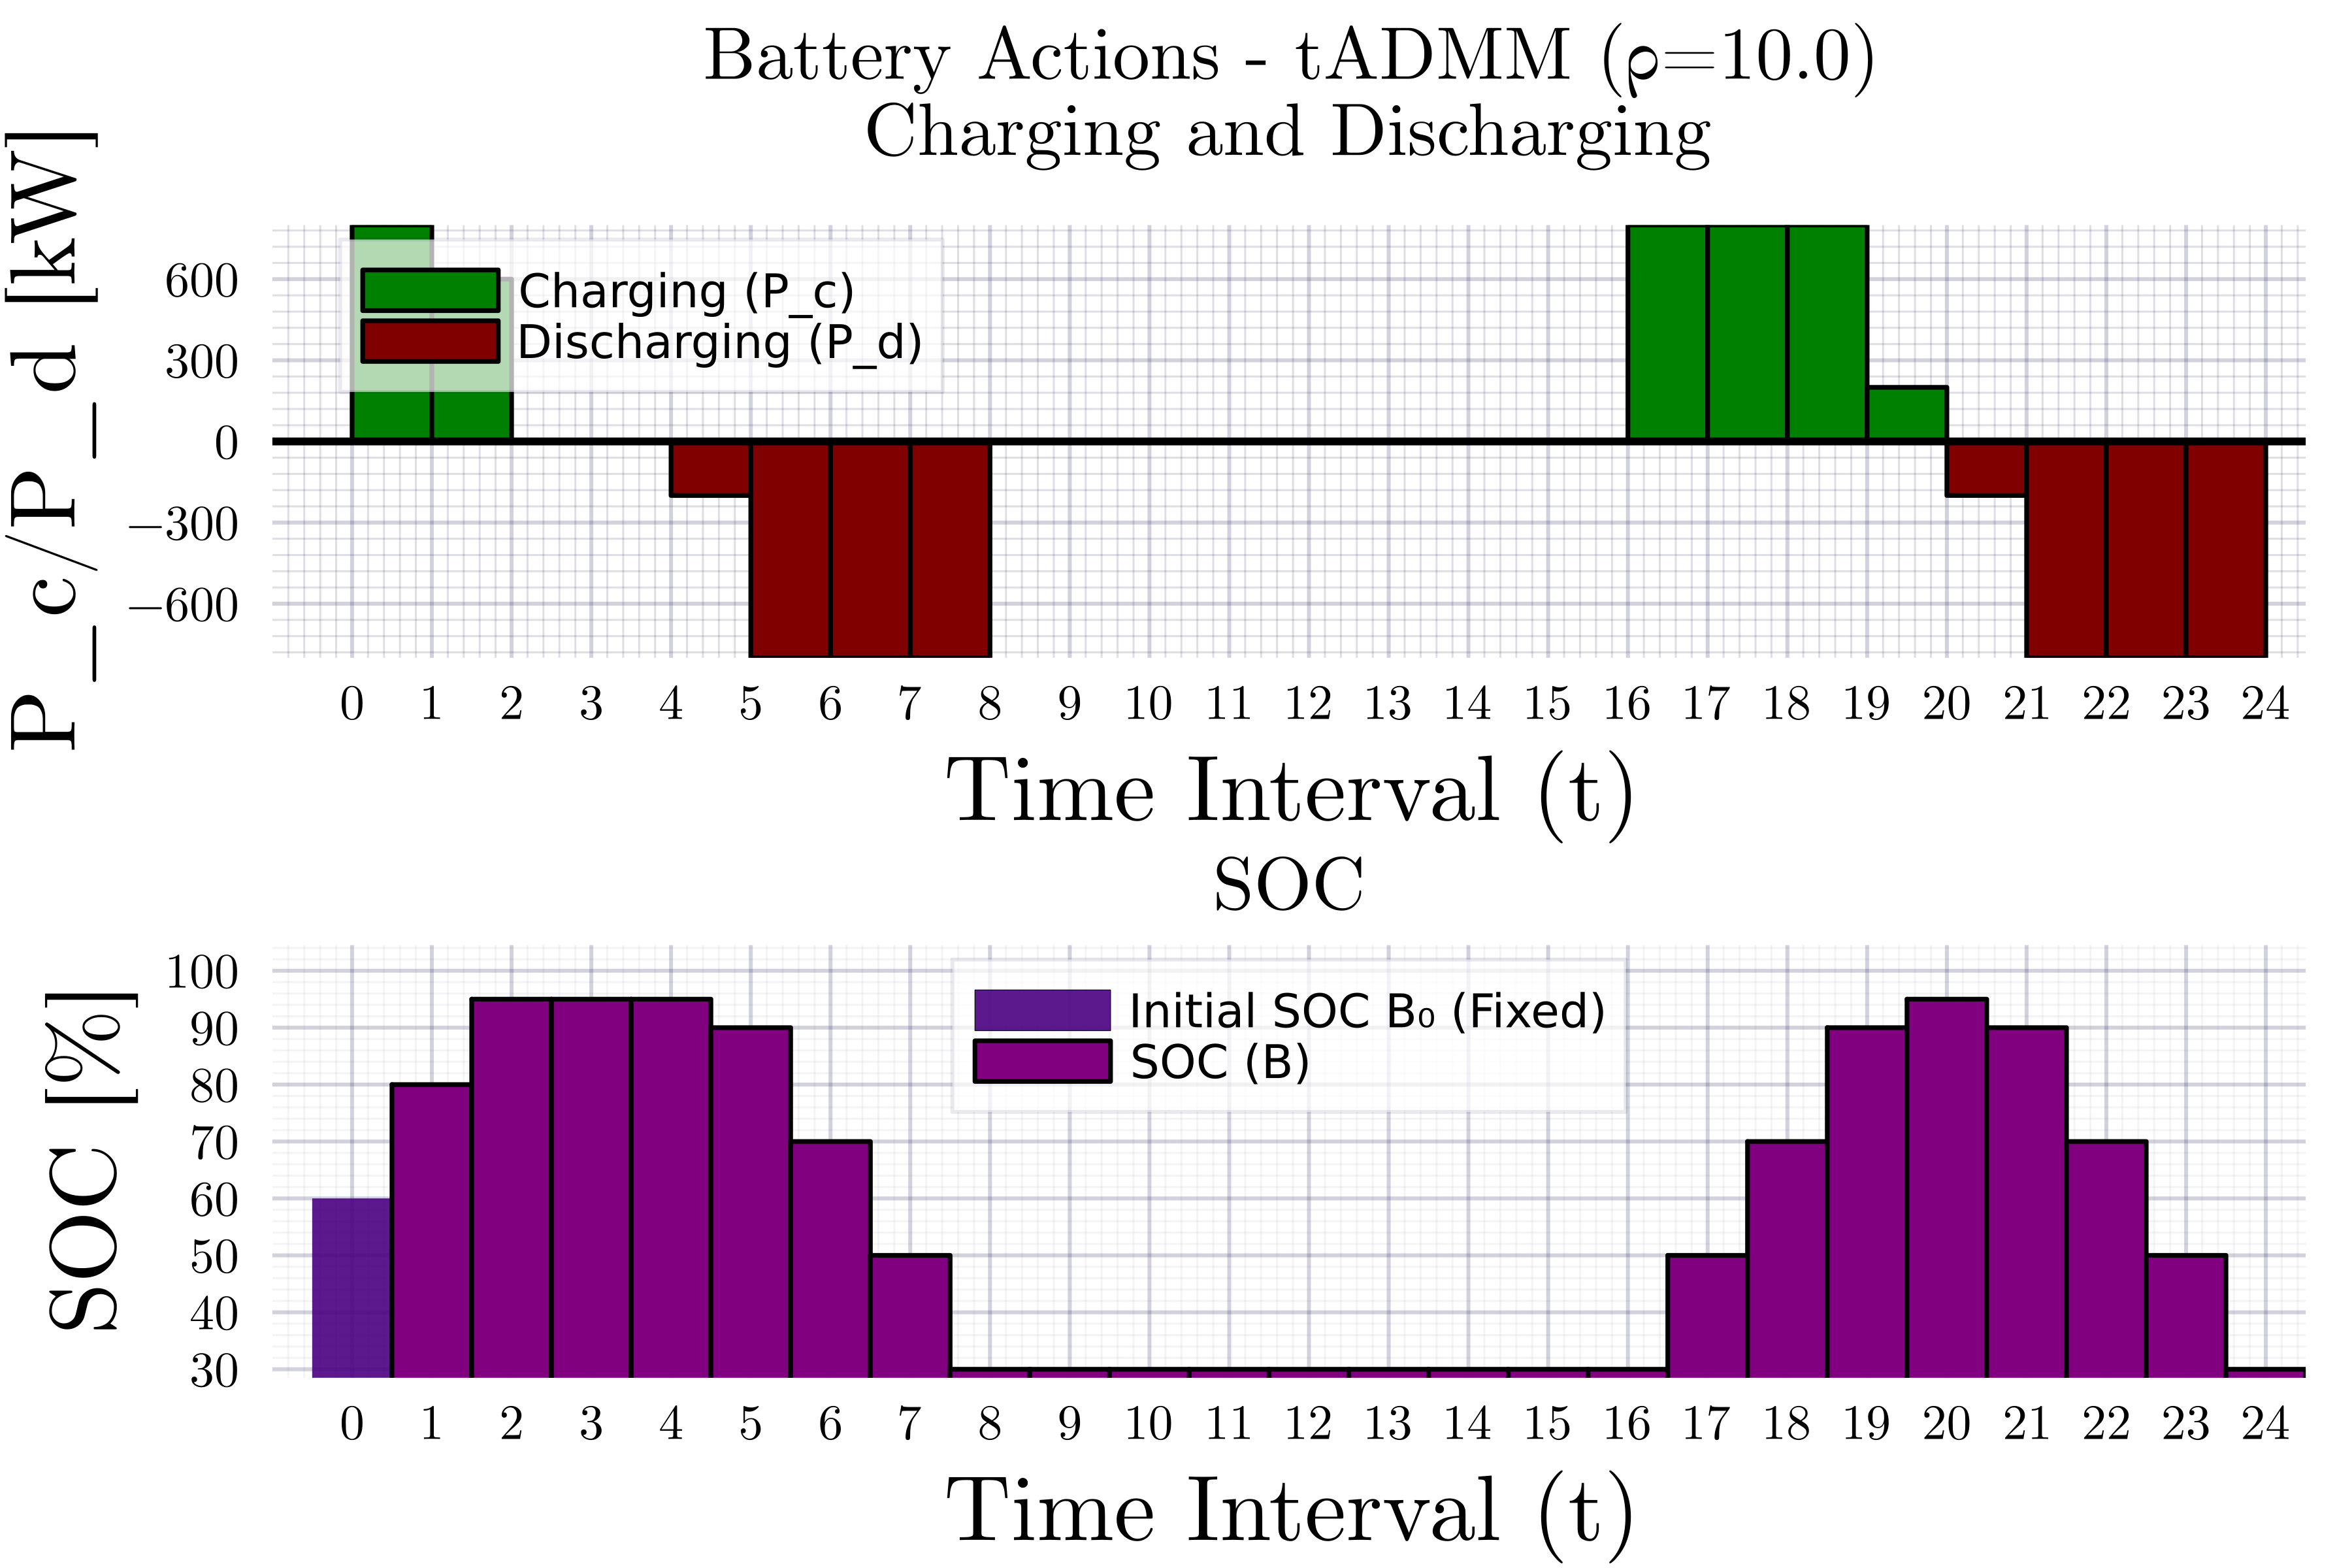
\includegraphics[width=0.7\textwidth]{figures/battery-actions-copper-plate-T24-tadmm.png}
    \caption{Battery power actions obtained using tADMM for copper plate MPOPF over 24-hour horizon. The solution converges to match the centralized optimal solution.}
    \label{fig:battery_actions_tadmm}
\end{figure}

Fig.~\ref{fig:convergence_curves} illustrates the convergence behavior of the tADMM algorithm, showing how the primal and dual residuals decrease over iterations until they satisfy the specified convergence tolerances ($\epsilon_{\text{pri}} = 10^{-3}$ and $\epsilon_{\text{dual}} = 10^{-3}$). The algorithm typically converges within a few dozen iterations, demonstrating good computational efficiency. The primal residual (consensus violation) decreases as the local SOC trajectories \textcolor{blue}{$\mathbf{B^{t_0}}$} converge to the global consensus \textcolor{red}{$\mathbf{\hat{B}}$}, while the dual residual tracks the stability of the consensus variable across iterations.

\begin{figure}[h]
    \centering
    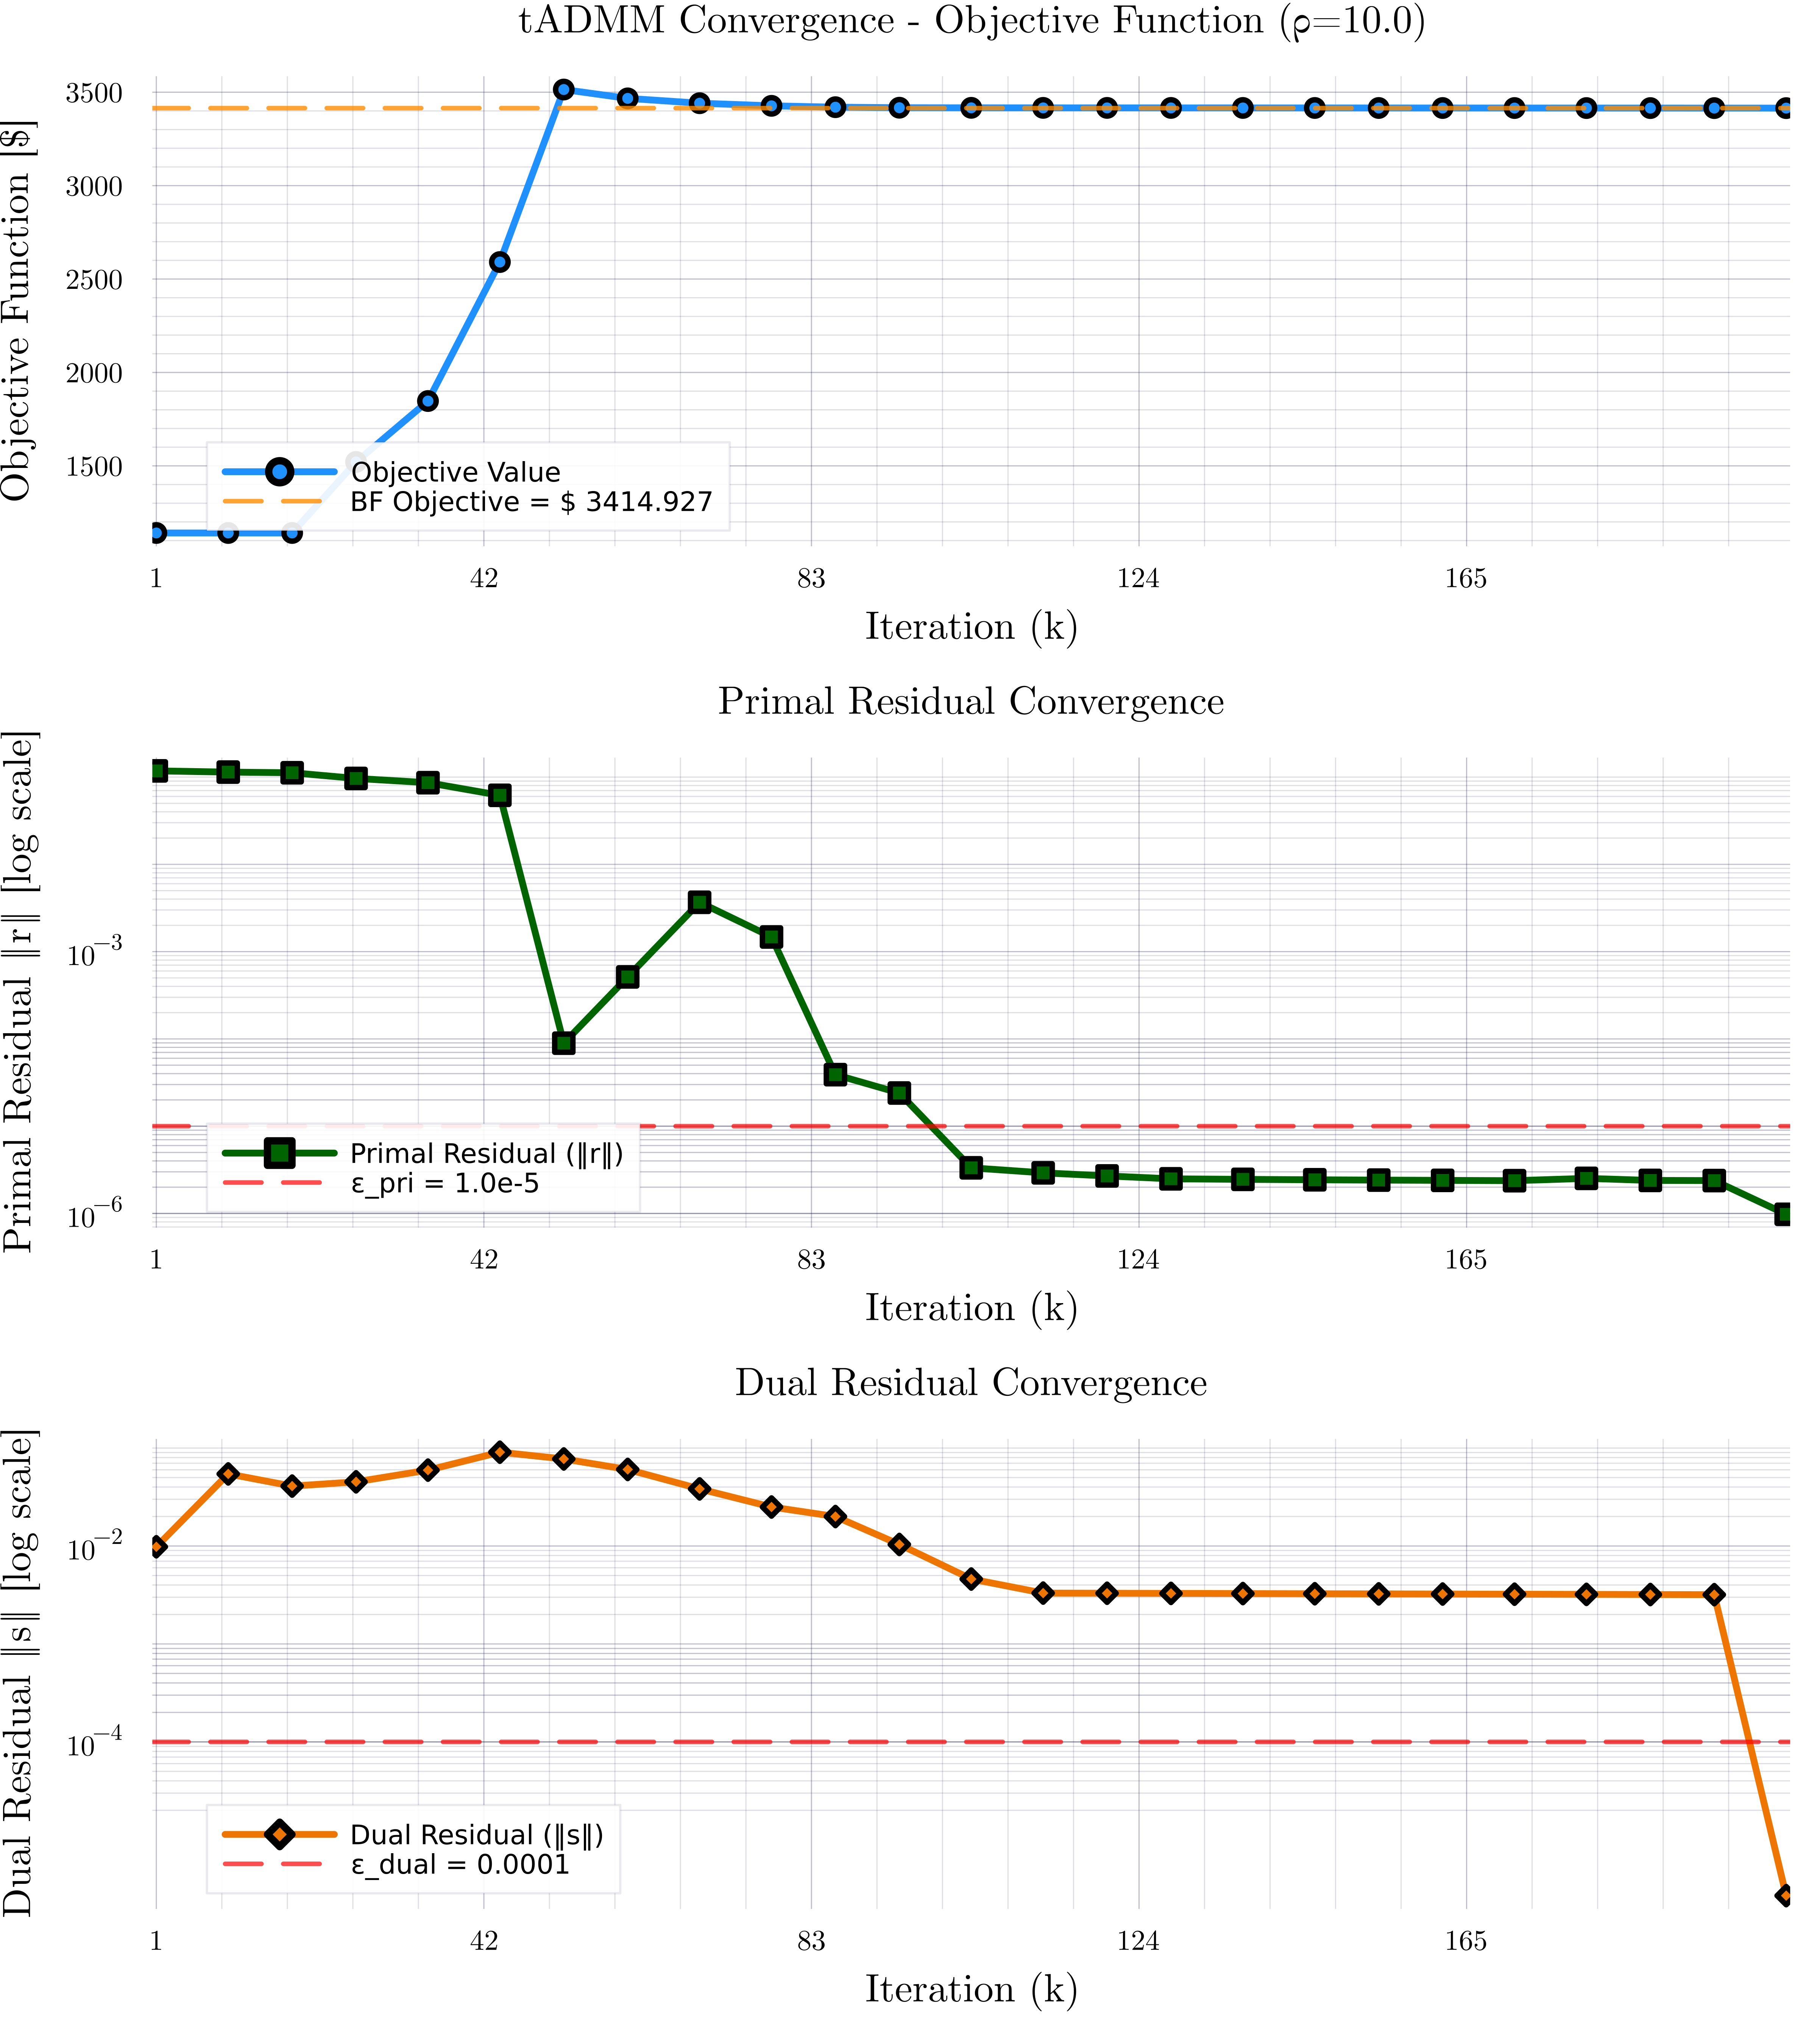
\includegraphics[width=0.7\textwidth]{figures/convergence-curves-copper-plate-T24-tadmm.png}
    \caption{Convergence curves showing primal and dual residuals for tADMM algorithm. Both residuals decrease monotonically and satisfy the convergence criteria.}
    \label{fig:convergence_curves}
\end{figure}

\subsection{Convergence Criteria}

The algorithm terminates when both residuals fall below specified thresholds:

\subsubsection{Convergence Criteria}

The algorithm terminates when both residuals fall below specified thresholds:

\textbf{Primal Residual (Consensus Violation):}

The primal residual measures how well the local SOC trajectories \textcolor{blue}{$\mathbf{B^{t_0}}$} agree with the global consensus \textcolor{red}{$\mathbf{\hat{B}}$}. A small primal residual indicates that all subproblems have converged to a consistent SOC trajectory.

\begin{align}
\|r^k\|_2 &= \left\| \text{vec}\left( \left\{ \textcolor{blue}{\mathbf{B^{t_0}}} - \textcolor{red}{\mathbf{\hat{B}}} \right\}_{t_0=1}^T \right) \right\|_2 \leq \epsilon_{\text{pri}}
\end{align}

\textbf{Dual Residual (Consensus Change):}

The dual residual measures how much the consensus variable \textcolor{red}{$\mathbf{\hat{B}}$} is changing between iterations. A small dual residual indicates that the consensus has stabilized.

\begin{align}
\|s^k\|_2 &= \rho \left\| \textcolor{red}{\mathbf{\hat{B}^k}} - \textcolor{red}{\mathbf{\hat{B}^{k-1}}} \right\|_2 \leq \epsilon_{\text{dual}}
\end{align}

\subsection{Algorithm Parameters}

\subsubsection{Objective Function Components}

The tADMM objective function for each subproblem $t_0$ consists of three terms:

\begin{align}
\text{Energy Cost:} \quad & C^{t_0} \cdot P_{\text{subs}}^{t_0} \cdot \Delta t \\
\text{Battery Quadratic Cost:} \quad & C_B \cdot \left(P_{B}^{t_0}\right)^2 \cdot \Delta t \\
\text{ADMM Penalty:} \quad & \frac{\rho}{2} \left\| B^{t_0} - \hat{B} + u^{t_0} \right\|_2^2
\end{align}

Where:
\begin{itemize}
    \item $C^{t_0}$: Energy price at time $t_0$ [\$/kWh]
    \item $C_B$: Battery quadratic cost coefficient [\$/kW$^2$/h] (typically $10^{-6} \times \min(C^t)$)
    \item $\rho$: ADMM penalty parameter
\end{itemize}

The battery quadratic cost term $C_B \cdot \left(P_{B}^{t_0}\right)^2$ serves as a regularization to:
\begin{enumerate}
    \item Prevent excessive battery cycling
    \item Encourage smoother power trajectories
    \item Improve numerical conditioning of the optimization problem
\end{enumerate}

\subsubsection{Algorithmic Parameters}

\begin{itemize}
    \item \textbf{Penalty Parameter}: $\rho$ (typically 0.1 to 10.0)
    \item \textbf{Primal Tolerance}: $\epsilon_{\text{pri}} = 10^{-3}$
    \item \textbf{Dual Tolerance}: $\epsilon_{\text{dual}} = 10^{-3}$
    \item \textbf{Maximum Iterations}: 1000
\end{itemize}

\subsection{Appendix: Full Variable and Parameter Definitions}

\subsubsection{System Bases}
\begin{align}
\text{kV}_B &= \frac{4.16}{\sqrt{3}} \text{ kV (phase-to-neutral)} \\
\text{kVA}_B &= 1000 \text{ kVA} \\
P_{\text{BASE}} &= 1000 \text{ kW} \\
E_{\text{BASE}} &= 1000 \text{ kWh per hour}
\end{align}

\subsubsection{SOC Bound Definitions}
\begin{align}
\underline{B} &= \text{SOC}_{\min} \cdot E_{\text{Rated}} \\
\overline{B} &= \text{SOC}_{\max} \cdot E_{\text{Rated}}
\end{align}

\subsubsection{Physical Interpretation}
\begin{itemize}
    \item $P_B[t] > 0$: Battery discharging (providing power to the system)
    \item $P_B[t] < 0$: Battery charging (consuming power from the system)
    \item $B[t]$: Battery state of charge at the end of period $t$
    \item $\underline{B} = \text{SOC}_{\min} \cdot E_{\text{Rated}}$: Lower SOC bound
    \item $\overline{B} = \text{SOC}_{\max} \cdot E_{\text{Rated}}$: Upper SOC bound
\end{itemize}

\subsection{Summary and Discussion}

The temporal ADMM (tADMM) approach provides an effective decomposition framework for solving multi-period optimal power flow problems with energy storage. The key advantages of this approach include:

\begin{itemize}
    \item \textbf{Parallelization}: Each time-step subproblem can be solved independently and in parallel, enabling computational speedup on multi-core processors or distributed computing platforms
    \item \textbf{Modularity}: The decomposition structure is flexible and can accommodate different network models (LinDistFlow, AC power flow, copper plate) without changing the temporal decomposition framework
    \item \textbf{Scalability}: The computational complexity scales more favorably with the number of time periods compared to solving the full centralized problem
    \item \textbf{Convergence guarantees}: For convex formulations, ADMM provides theoretical convergence guarantees to the global optimum~\cite{admm_boyd_website, admm_cmu_notes}
\end{itemize}

The numerical results demonstrate that tADMM successfully decomposes the temporal coupling through battery SOC while maintaining solution optimality. The algorithm converges within a reasonable number of iterations, and the final solution matches the centralized optimal solution within the specified tolerances. This validates the effectiveness of the consensus-based decomposition for handling temporal coupling in MPOPF problems.

Future extensions of this work will focus on:
\begin{itemize}
    \item Applying tADMM to larger distribution networks with multiple batteries and renewable energy sources
    \item Investigating adaptive penalty parameter selection strategies to improve convergence speed
    \item Extending the framework to handle nonconvex AC power flow formulations
    \item Integrating spatial decomposition techniques with temporal decomposition for enhanced scalability
\end{itemize}

